\section{Objektdetektion}

Das folgende Kapitel befasst sich mit den ersten beiden Schritten in der automatisierten Analyse der Grabungsfotos: der Erkennung der Schiefertafeln und ihrer Extraktion aus dem Gesamtbild.\\
Zunächst werden verschiedene Möglichkeiten der Erkennung präsentiert und diskutiert. Der Schwerpunkt liegt hier auf dem schlussendlich umgesetzten Verfahren.
Abschließend wird das mit der Tafeldetektion verbundene Ausschneiden der gefundenen Tafeln aus dem Gesamtbild vorgestellt.

\subsection{Detektionsverfahren}

Aus den Anforderungen der Aufgabenstellung lässt sich als erster Arbeitsschritt die Detektion der Tafeln ableiten. Die wichtigste Prämisse ist dabei, dass Falsch-Negative, also nicht erkannte Tafeln, vermieden werden. Grund dafür ist, dass diese für die weitere Bearbeitung komplett verloren sind. Falsch-Positive sollten ebenfalls weitestgehend ausgeschlossen werden. Diese können jedoch in späteren Bearbeitungsschritten, vor allem der Texterkennung, erkannt und aussortiert werden. Daher ist dieses Kriterium von niedrigerer Priorität.
Dieses Kapitel wird sich daher verschiedenen Verfahren widmen, mit denen rechteckige, beschriftete Objekte erkannt werden können. Diese Verfahren werden vorgestellt und ihre Ergebnisse in einer ersten, explorativen Umsetzung präsentiert. Anschließend wird begründet, warum diese Verfahren im Rahmen des Projektes nicht nicht zum Einsatz kommen. Final wird dann das Kontur-basierte Erkennungsverfahren erläutert, mit dem die besten Ergebnisse erzielt wurden.

%das Kapitel wird aus einer Kurzvorstellung der einzelnen Ansätze bestehen, die in Frage kamen und ausprobiert wurden
%In der Tiefe wird sich anschließend mit dem letztlich umgesetzten Verfahren, basierend auf \verb|cv2.contours|, auseinandergesetzt.

\subsubsection{Feature Detection}

was ist feature detection?
wie funktioniert sie?
was war die Idee hinter dem Ansatz?
Wie sehen die Ergebnisse aus?

\subsubsection{CNN}

hier werden CNNs vorgestellt
was sind CNNs?
Was können sie, wie funktionieren sie?
Warum habe ich sie ausprobiert, was war die Idee dahinter?
Warum habe ich nicht selbst trainiert?
Wie sehen die Ergebnisse aus?

\subsubsection{Contours}

\verb|Cv2.Contours| basiert auf einem Algorithmus, der Punkte gleicher Farbe und Intensität umrandet \cite{suzuki}. Das Resultat ist eine Liste von Punkten, die ein geschlossenes Polygon ergeben. Die gefundenen Konturen können mit einer Hierarchie versehen werden, bei der Konturen, die sich innerhalb anderer Konturen befinden, als deren \glqq Kinder\grqq gelten. Das Verfahren ist darauf ausgelegt, auf binäre Bilder angewendet zu werden. Die Implementierung in OpenCV unterscheidet in Nullwerte und Nicht-Nullwerte \cite{opencvcontours}. Nicht-binäre Bilder werden also automatisch binarisiert. Für die Erzielung optimaler Ergebnisse kommt dem Binarisierungsverfahren allerdings eine große Bedeutung zu.
Auf Basis dieses Algorithmus lässt sich Detektionsverfahren aufbauen, das Objekte, die sich vom Hintergrund der Bilder abheben, zu erkennen. Die Herausforderung besteht, nach diesem Ansatz, in zwei Punkten: Erstens muss die Binarisierung so erfolgen, dass eine möglichst saubere Trennung von Vordergrund (Objekten) und Hintergrund (vor allem Erde) der Bilder stattfindet und zweitens müssen aus den gefundenen Vordergrundobjekten diejenigen ausgewählt werden, die als Tafeln in Frage kommen. Wie bereits erwähnt hat dabei die Vermeidung Falsch-Negativer eine höhere Priorität als die von Falsch-Positiven. Bei der Binarisierung haben sich zwei Wege als praktikabel herausgestellt, die im Folgenden beide präsentiert werden sollen. Im Flowchart sind die Abläufe der Rechtecksdetektion schematisch dargestellt (Vgl. Abb.\ref{fig:flowrectdetect}).
\begin{figure}[h!]
\centering
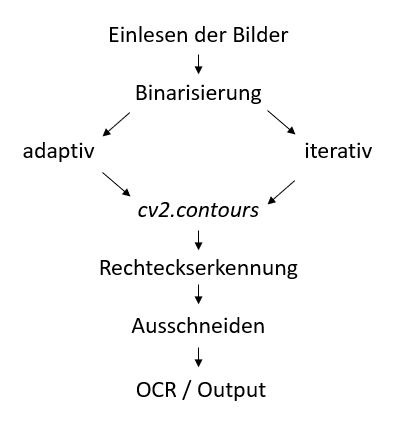
\includegraphics[width =0.5\textwidth]{flowchart_cont.PNG}
\caption{Flowchart Rechteckserkennung.}
\label{fig:flowrectdetect}
\end{figure}

\subsubsection*{Adaptive Binarisierung}

Das einfachste Verfahren der Binarisierung eines Bildes besteht darin, einen Threshold, also einen Grenzwert festzulegen. Dieser muss auf der Spanne der Farbwerte, also zwischen 0 und 255 liegen.  Farbwerte unterhalb dieses Thresholds werden zu Nullen, Farbwerte darüber zu Einsen. Das Ergebnis ist ein reines Schwarz-Weiß-Bild. Bei komplexen Szenerien, wie den Grabungsfotos, ist dieses Verfahren jedoch zu einfach. So kann ein Foto beispielsweise stark unterschiedliche Beleuchtung, wie direktes Sonnenlicht und Schatten, enthalten. Eine Differenzierung innerhalb dieser Zonen ist so nicht möglich (Vgl. Abb. \ref{fig:threshold}.\\
\begin{figure}[h!]
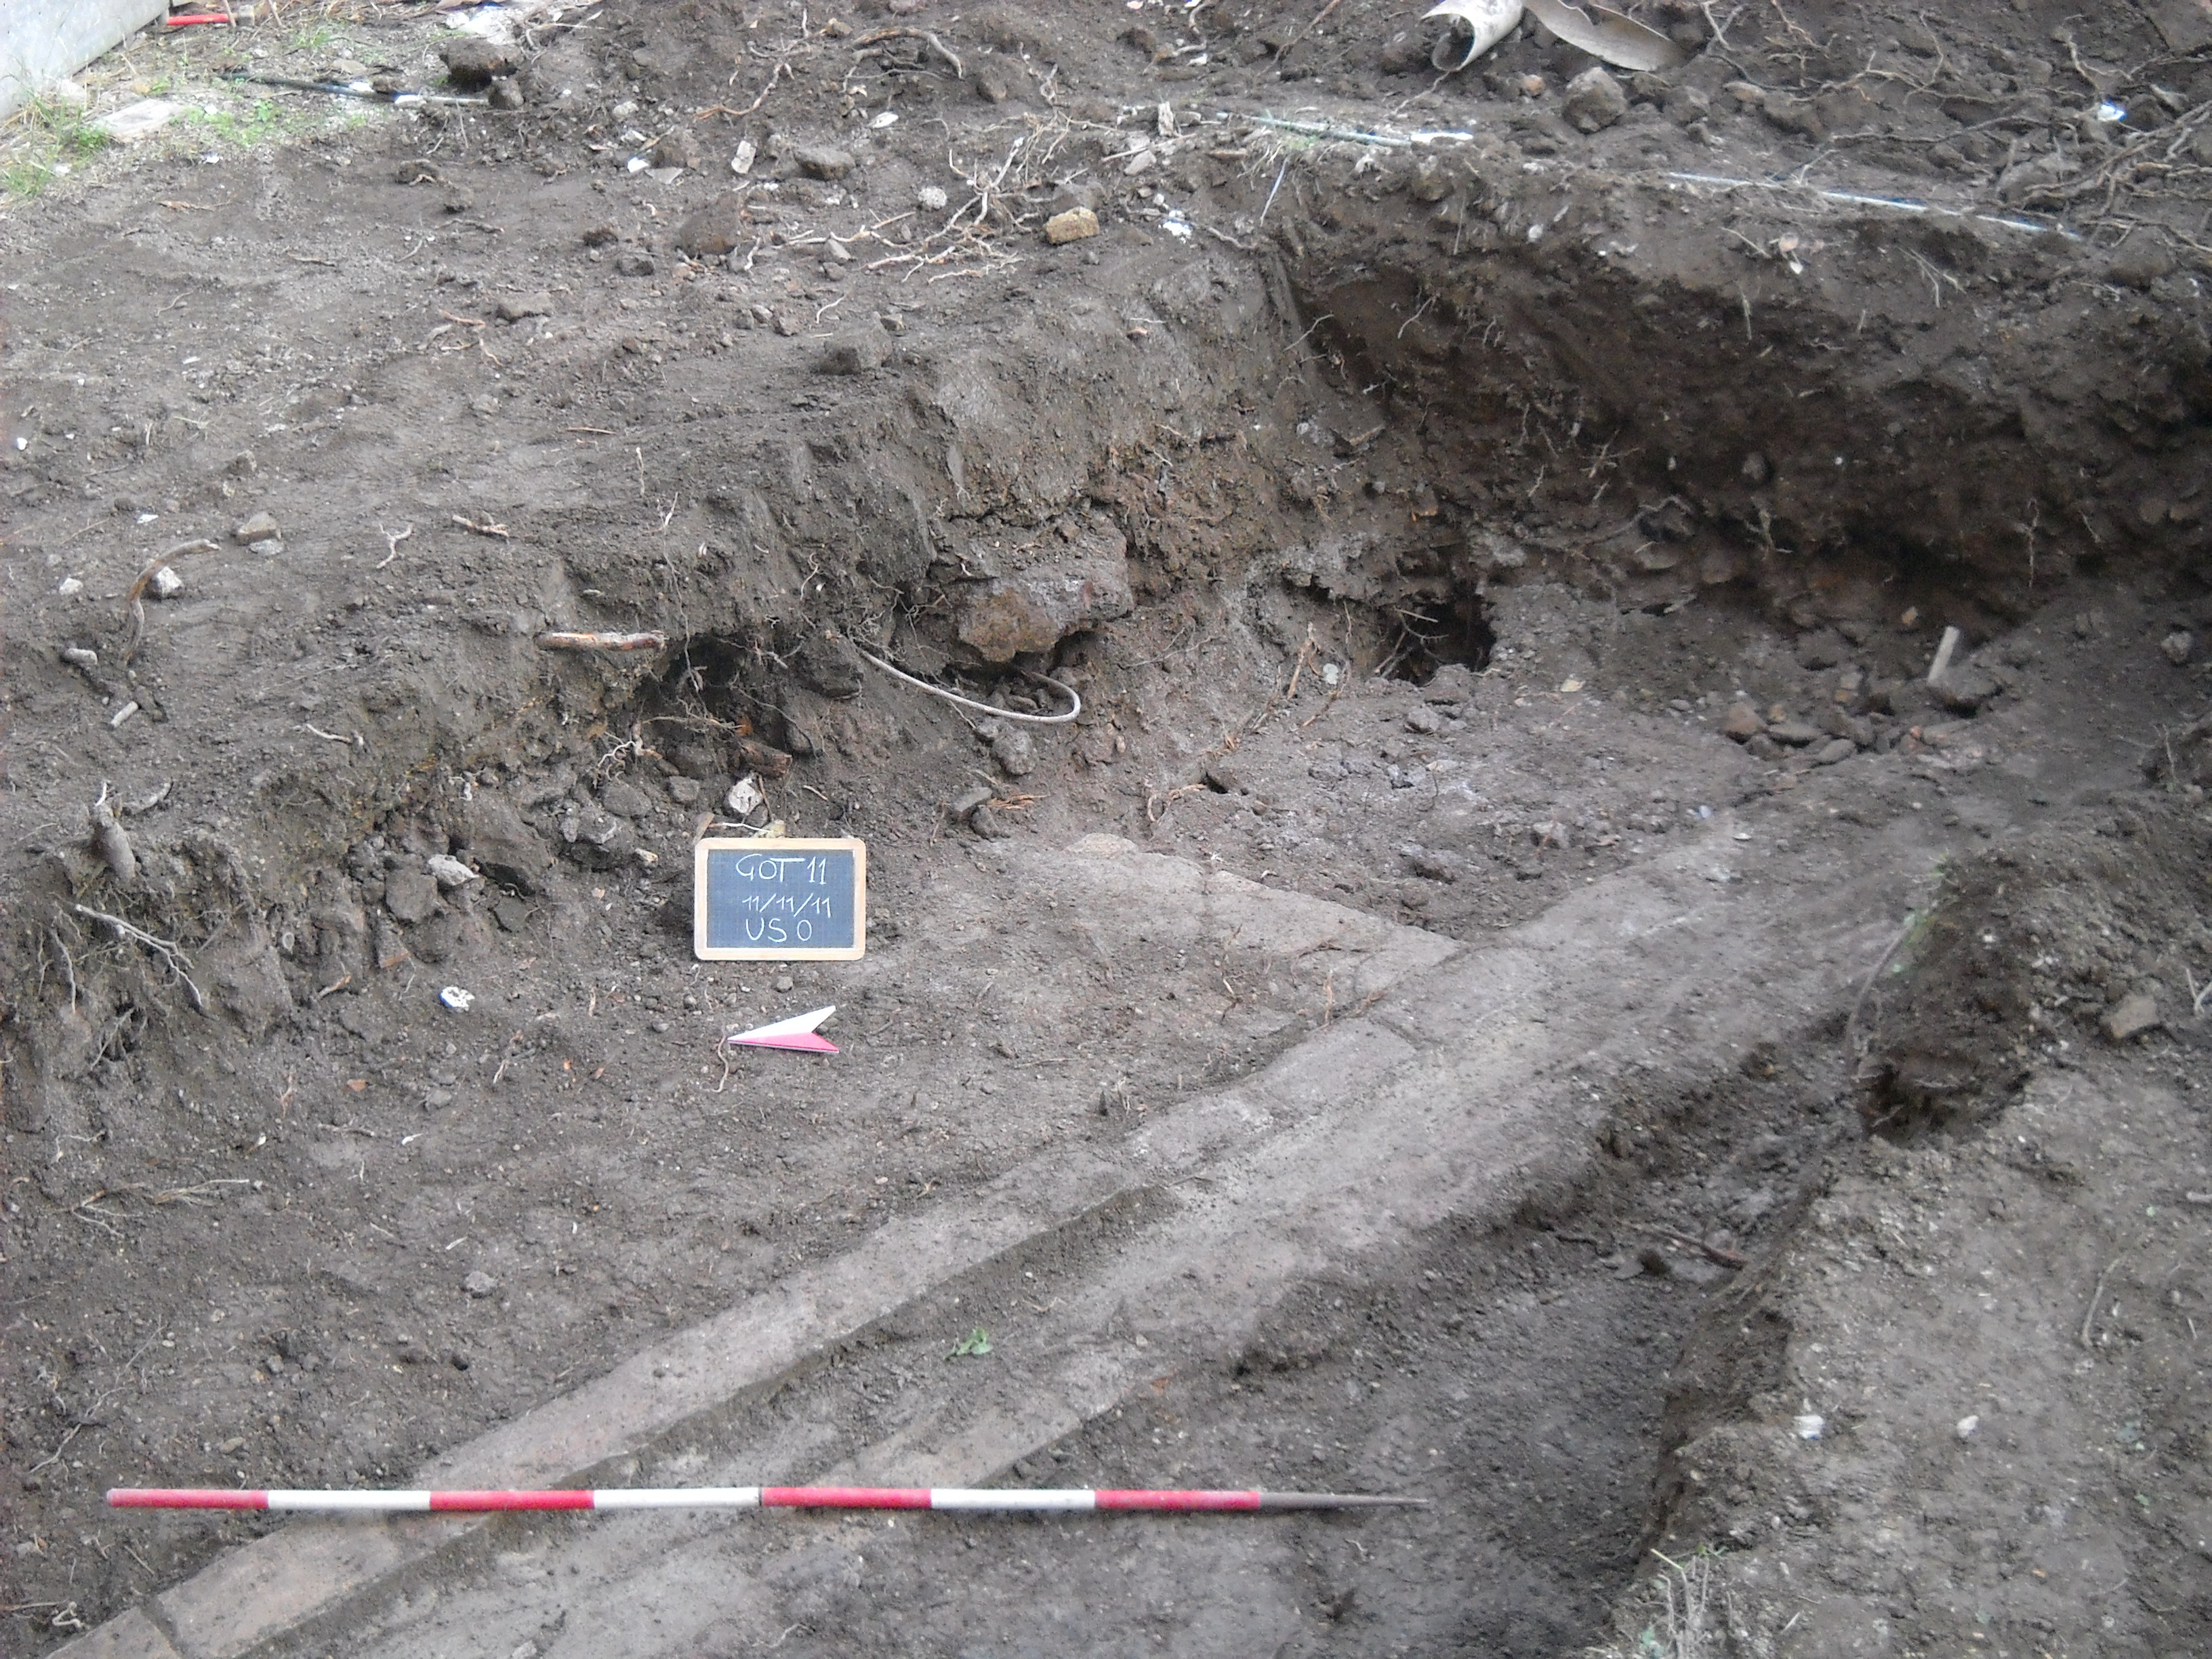
\includegraphics[width =0.5\textwidth]{catacom_1020.JPG}
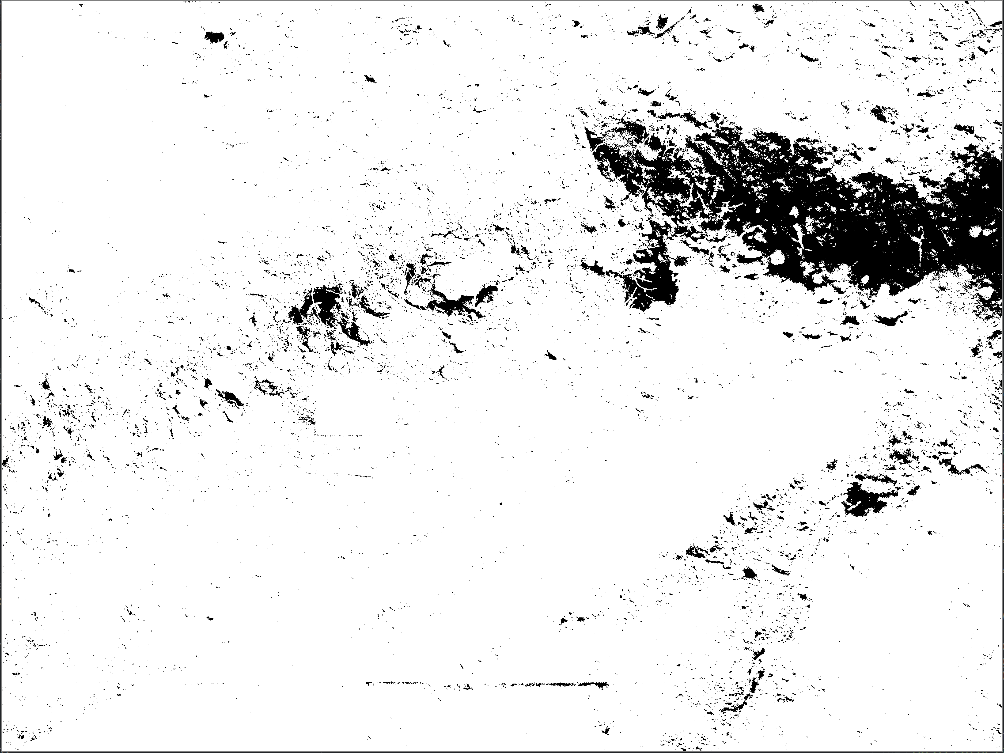
\includegraphics[width =0.5\textwidth]{thresh60.png}
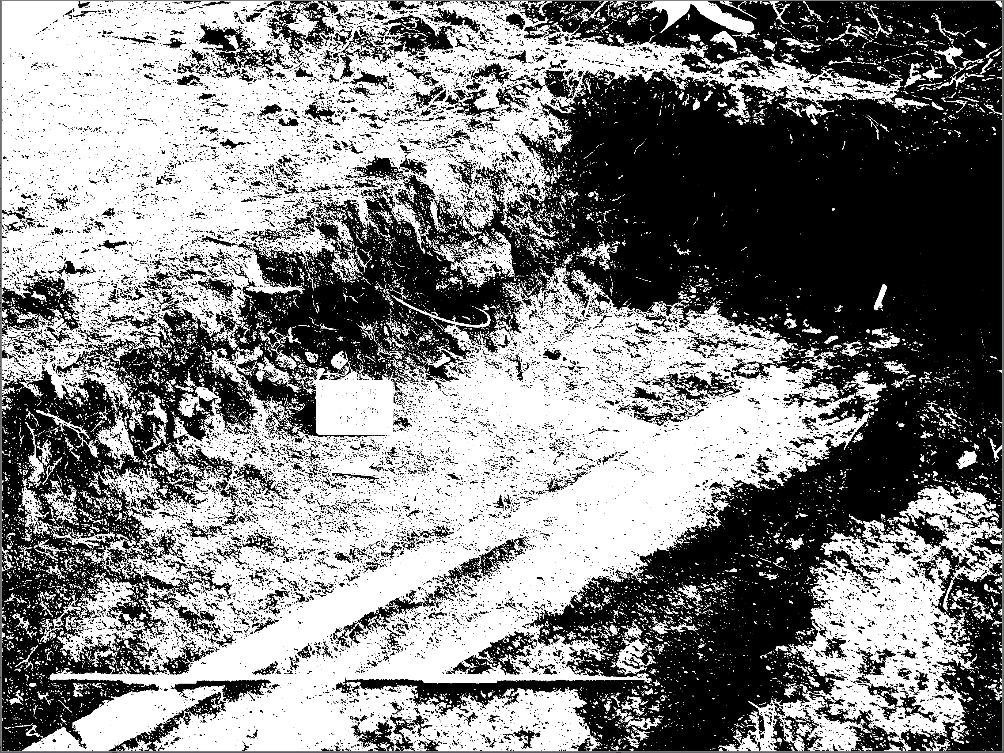
\includegraphics[width =0.5\textwidth]{thresh125.png}
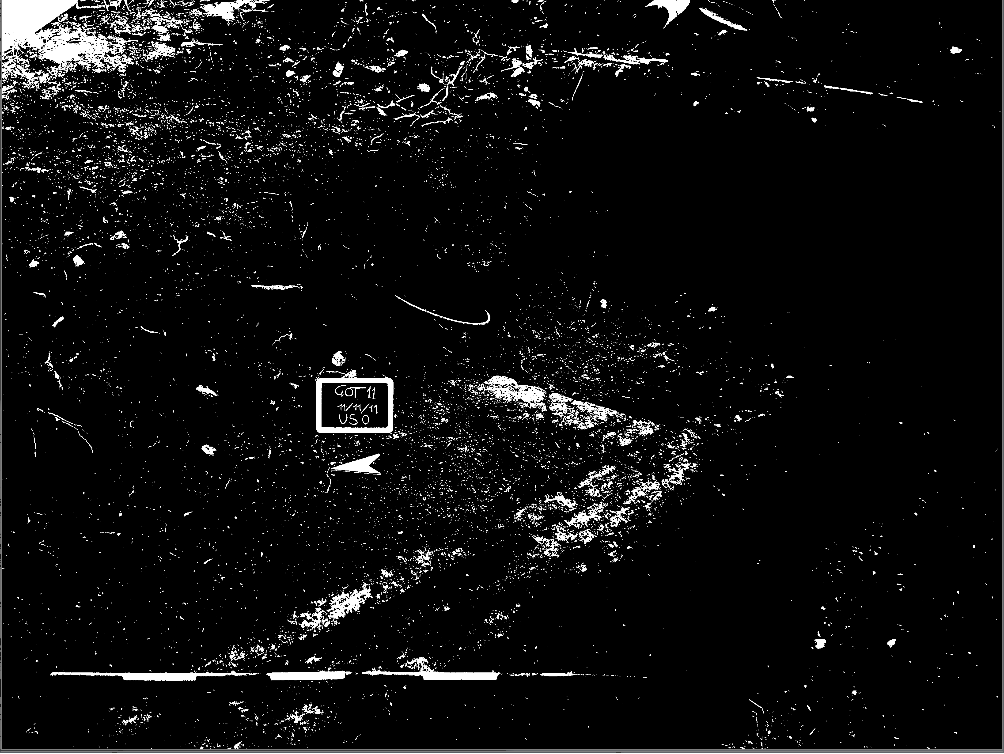
\includegraphics[width =0.5\textwidth]{thresh185.png}
\caption{Grabungsfoto im Original (o.l.), mit niedrigem (60, o.r.), mittlerem (125, u.l.) und hohem (185, u.r.) Threshold.}
\label{fig:threshold}
\end{figure}
Eine Lösung für dieses Problem ist die Anwendung eines adaptiven Thresholds \cite{opencvadaptivethresholdopencvadaptivethreshold}): Statt global, über das gesamte Bild, einen Grenzwert festzulegen, können lokale Grenzwerte errechnet werden. Die Größe des lokalen Ausschnittes sowie das exakte Verfahren können dabei frei gewählt werden. In diesem Fall wird für die Binarisierung ein Gauss-Verfahren auf einen Kernel von 11 x 11 Pixeln angewendet. Die Beleuchtung oder Farbunterschiede innerhalb des Bildes können so ausgeglichen werden (Vgl. Abb. \ref{fig:adaptivethreshold}).
\begin{figure}[h!]
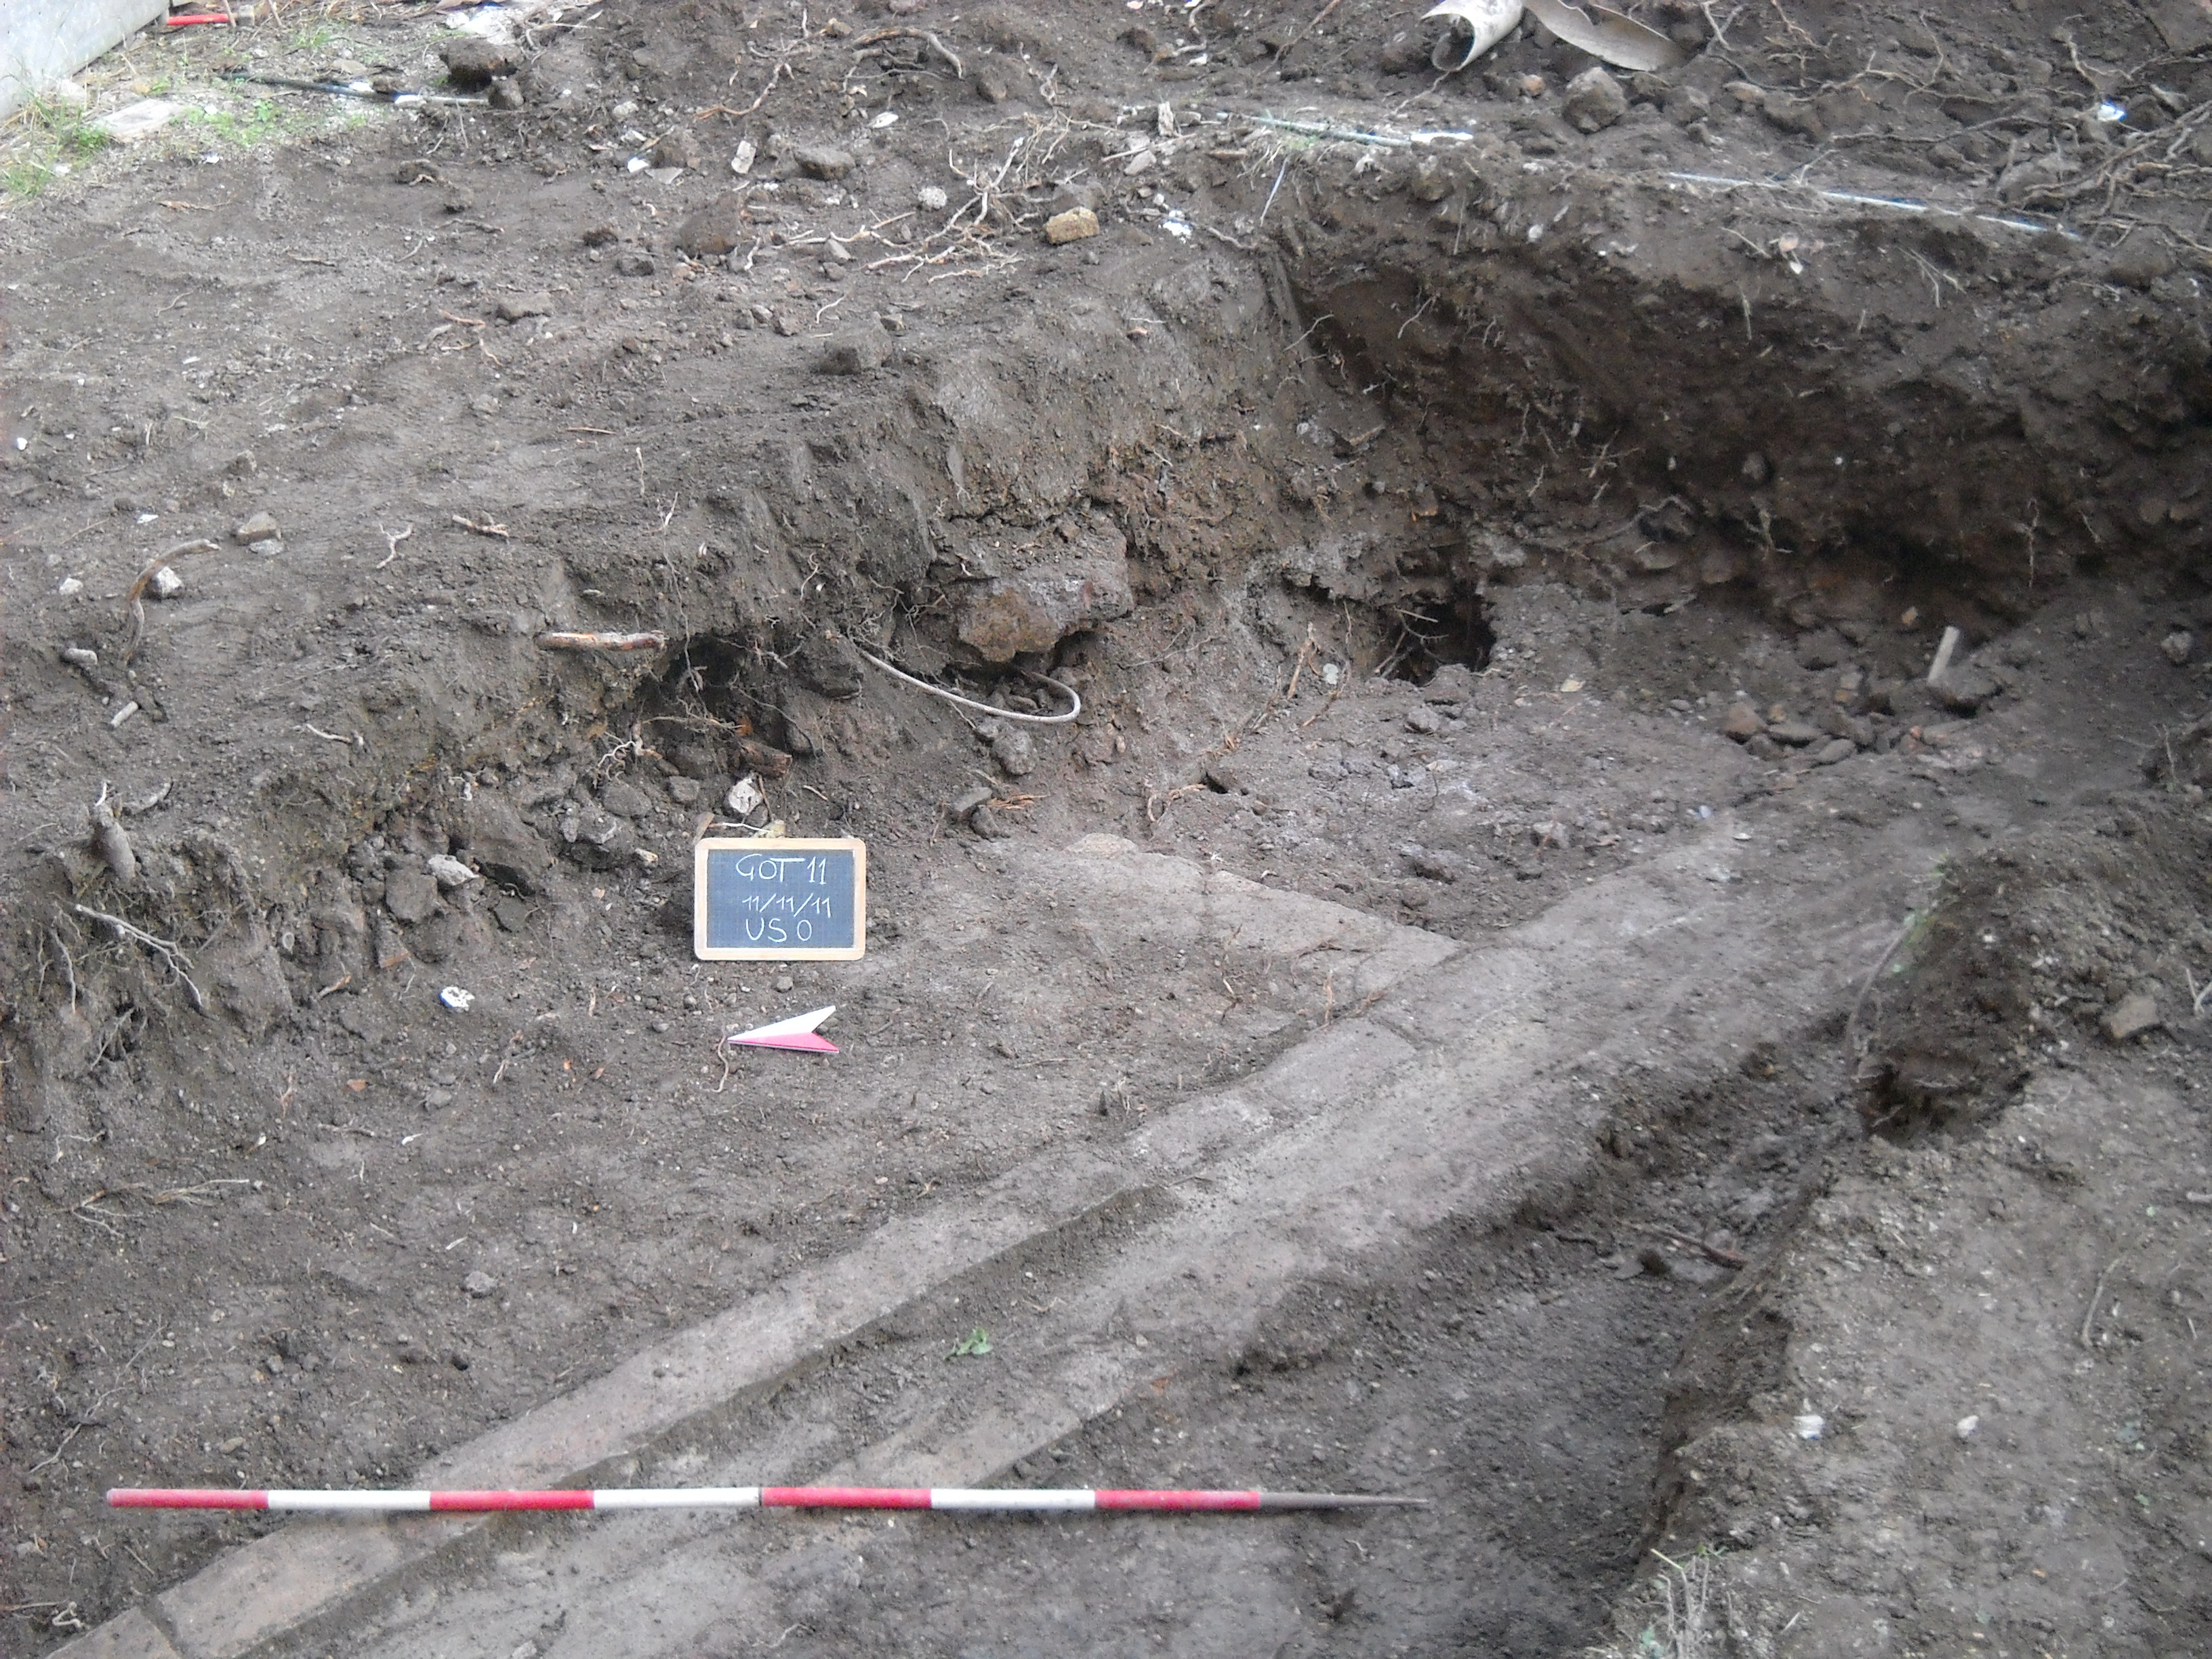
\includegraphics[width =0.5\textwidth]{catacom_1020.JPG}
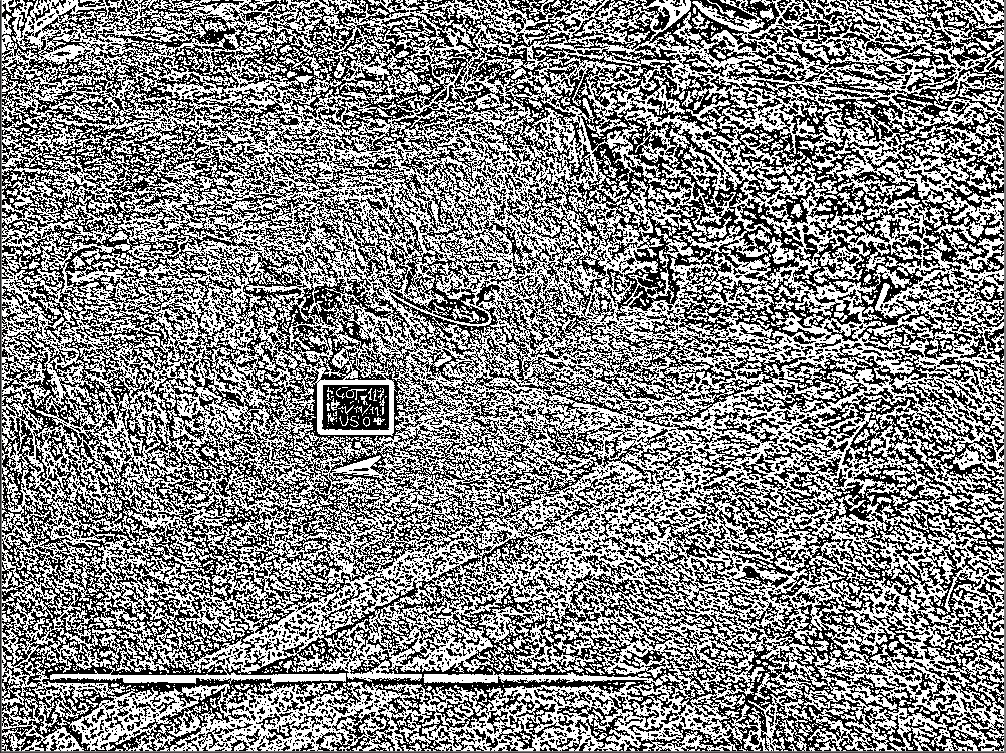
\includegraphics[width =0.5\textwidth]{adaptivethreshold.png}
\caption{Grabungsfoto im Original sowie mit adaptivem Threshold.}
\label{fig:adaptivethreshold}
\end{figure}
Vor der Binarisierung muss das Bild in ein Grauskala-Bild umgewandelt verkleinert\footnote{Genauer: Der längere Bildrand wird auf 1000 Pixel reduziert, der kürzere entsprechend angepasst. Die Grabungsfotos haben in der Regel eine Auflösung von 3264 x 2448 Pixeln. Es findet also eine Reduktion auf ca. $\frac{1}{9}$ der Fläche statt. Bilder kleiner als 1000 Pixel würden theoretisch auf 1000 Pixel vergrößert werden. Da für die hier beschriebenen Prozesse und vor allem für die Texterkennung später aber eine gewisse Bildqualität erforderlich ist, ist von diesem Fall nicht auszugehen.}. Das verbessert die Genauigkeit der Detektion und verringert die zu verarbeitende Datenmenge, wodurch der Prozess beschleunigt wird. Die Verkleinerung des Bildes ist allerdings ein Prozess, der später rückgängig gemacht werden muss, um Datenverlust bei der Texterkennung zu verhindern.

\subsubsection*{Iterative Binarisierung}

Die adaptive Binarisierung bringt einige Nachteile mit sich. So ist hier die Erkennung von Falsch-Positiven relativ hoch. Die Konturen werden auf einem verkleinerten Bild gesucht und müssen später auf Originalgröße skaliert werden, was ein verlustbehafteter Prozess ist. Daher gibt es einen zweiten Ansatz, hier als iterativer Ansatz bezeichnet. Die Grundidee besteht darin, das Bild mit einem globalen Threshold zu binarisieren. Die Problematik davon wurde bereits diskutiert: Bei großen Beleuchtungsunterschieden oder sehr hellen oder dunklen Objekten auf dem Bild werden ganze Bereiche durch den Threshold von der weiteren Bearbeitung ausgeschlossen. Der iterative Ansatz sieht daher vor, den Threshold von 20 auf 200 in Fünferschritten zu erhöhen. Dadurch entstehen pro Foto 37 binäre Bilder, auf die die Konturenerkennung angewendet werden kann. Auf jedem dieser Bilder können mehrere mögliche Tafeln erkannt werden\footnote{Die eigentliche Tafelerkennung wird erst im folgenden Abschnitt beschrieben. Da die dort gewonnenen Informationen nicht, wie beim adaptiven Ansatz, an das Hauptprogramm übergeben, sondern innerhalb der Funktion des iterativen Ansatzes weiter verarbeitet werden, ist hier ein Vorgriff nötig.}. Der nächste Schritt besteht also darin, aus diesen möglichen Tafeln die auszuwählen, die am wahrscheinlichsten tatsächlich eine ist. In diesem Kontext wird eine Grundannahme getroffen: Es wird davon ausgegangen, dass in dem Bereich, in dem auf den meisten der 37 Bilder eine Tafel vermutet wird, sich tatsächlich eine Tafel befindet. Alle anderen werden als Falsch-Positive betrachtet. Diese Annahme beruht auf zwei Faktoren: Erstens hat sich gezeigt, dass Objekte, die keine Tafeln sind, aber als solche erkannt werden können -- beispielsweise Fenster, Türen oder Plakate -- nur unter wenigen Thresholds als solche eingeordnet werden. Das liegt unter anderem darin begründet, dass die Tafeln einen hellen Holzrahmen und eine dunkle Innenfläche haben, was zum maximalen Kontrasten führt. Zweitens werden durch eben diesen Rahmen in mittleren Threshold-Bereichen die Tafeln zweimal erkannt: Einmal an der Außenkante und einmal an der Innenkante des Rahmens. Dadurch häuft sich die Detektion möglicher Tafeln in diesem Bereich.
Basierend auf dieser Annahme wird auf alle mögliche Tafeln immer paarweise die \verb|intersection_over_union| angewendet. Dieser Algorithmus basiert auf dem Jaccard-Koeffizienten zur Berechnung der Ähnlichkeit zweier Mengen \cite{intersectionoverunion}. Der Koeffizienten wird errechnet, indem die Schnittmenge durch die Vereinigungsmenge geteilt wird. Das Ergebnis liegt zwischen 0 und 1. Je mehr es sich der 1 annähert, desto ähnlicher sind die Mengen. Diese Berechnung lässt sich auch auf die Rechtecke, mit denen die möglichen Tafeln verortet werden, anwenden (Vgl. Abb. \ref{fig:jaccard}).

\begin{figure}[h!]
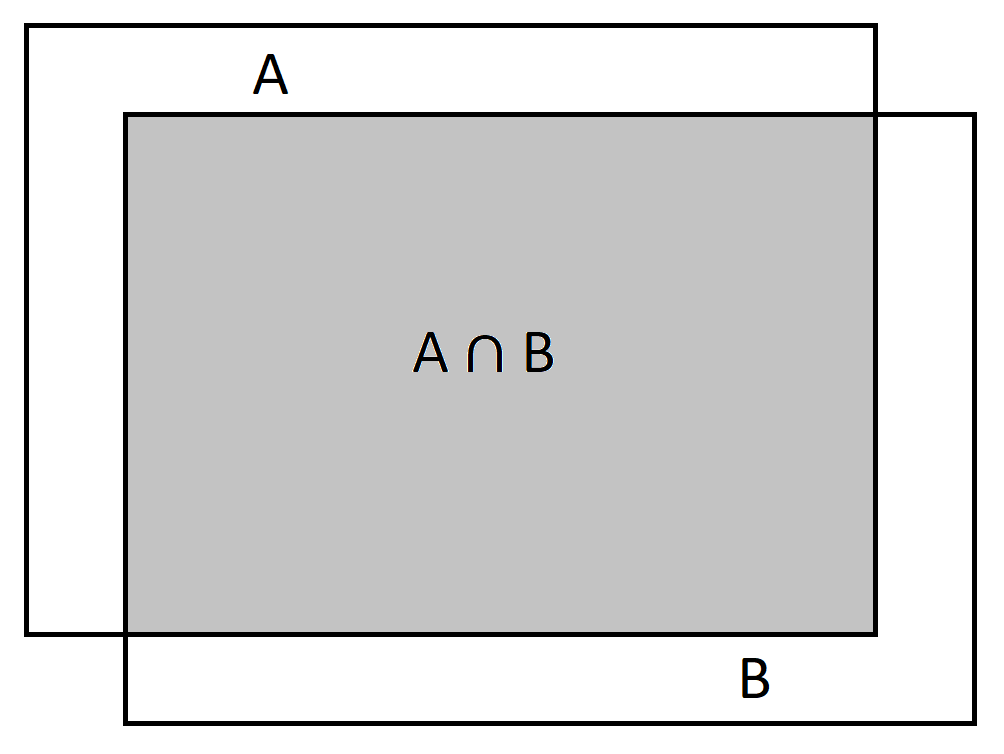
\includegraphics[width =0.5\textwidth]{schnittmenge.png}
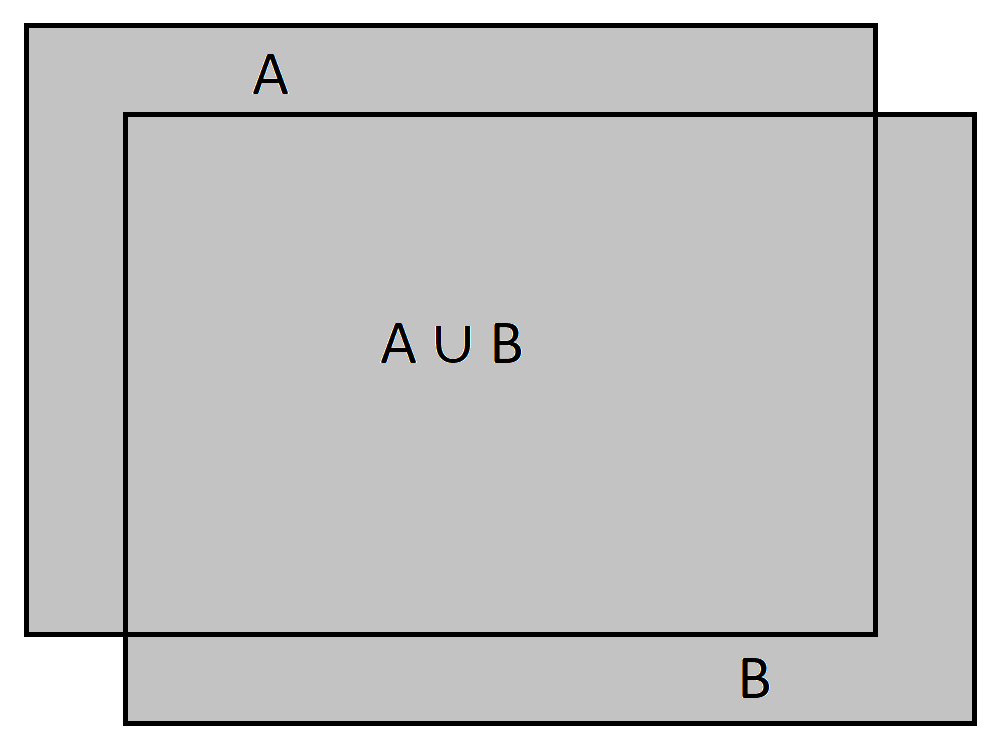
\includegraphics[width =0.5\textwidth]{vereinigungsmenge.png}
\caption{Schnittmenge und Vereinigungsmenge.}
\label{fig:jaccard}
\end{figure}

Zweispurigkeit der Ansätze: iterativ und adaptiv. Erklären warum.
\verb|rect_detect| als Finale, in dem die beiden Ansätze wieder zusammengeführt werden

\subsection{Cropverfahren}

Was ist die Aufgabe beim Crop?
Worin liegen hier die Schwierigkeiten?
Auch hier wieder Zweispurigkeit der Ansätze erklären

\subsubsection{simple crop}

Was ist die Idee?
Wie wurde sie umgesetzt?
Wo liegen die Probleme?

\subsubsection{Hough}

Was ist die Idee?
Wie wurde sie umgesetzt?
Wo liegen die Probleme?

\subsection{Zusammenfassung}
evtl zusammenfassen wie vorgegangen wurde, warum dieser Weg gut ist und was das Wichtigste Ergebnis ist